\emph{On note $F$ l'évènement \og le véhicule est un fourgon \fg{} et $B$ l'évènement \og le véhicule est en bon état \fg. On a
$P(F) = 0,6$, $P_F(B) = 0,5$ et $P(B) = 0,66$. On note $x = P_{\overline{F}}(B)$.}

\begin{enumerate}
	\item La somme des probabilités issues d'un même n{\oe}ud vaut 1 :
	
	$P\left(\overline{F}\right) = 1 - 0,6 = 0,4$ et $P_F\left(\overline{B}\right) = 1 - 0,5 = 0,5$.

	\begin{center}
		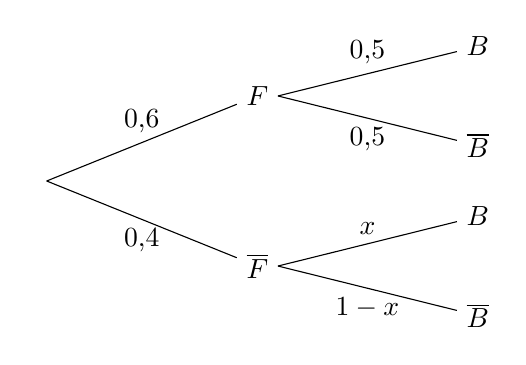
\begin{tikzpicture}[x=2.8cm, y=0.9cm]
			
			\node (root) at (0,0) {};
			\node (F) at (1,1.2) {$F$};
			\node (Fb) at (1,-1.2) {$\overline{F}$};
			\node (B1) at (2,1.9) {$B$};
			\node (B1b) at (2,0.5) {$\overline{B}$};
			\node (B2) at (2,-0.5) {$B$};
			\node (B2b) at (2,-1.9) {$\overline{B}$};
			
			\draw (root.east) -- (F) node[pos=0.5,above] {0,6};
			\draw (root.east) -- (Fb) node[pos=0.5,below] {0,4};
			
			\draw (F.east) -- (B1) node[pos=0.5,above] {0,5};
			\draw (F.east) -- (B1b) node[pos=0.5,below] {0,5};
			\draw (Fb.east) -- (B2) node[pos=0.5,above] {$x$};
			\draw (Fb.east) -- (B2b) node[pos=0.5,below] {$1-x$};
		\end{tikzpicture}
	\end{center}

	\item
	La probabilité que le véhicule choisi soit un fourgon en bon état est $P(F \cap B)$.
	
	$P(F \cap B) = P(F) \times P_F(B) = 0,6 \times 0,5 = 0,3$.

La probabilité que le véhicule choisi soit un fourgon en bon état est égale à $0,3$.
	\item On cherche la probabilité conditionnelle $P_B(F)$ :
	\[P_B(F) = \dfrac{P(F \cap B)}{P(B)} = \dfrac{0,3}{0,66} = \dfrac{30}{66} = \dfrac{5}{11}.\]
	Sachant que le véhicule choisi est en bon état, la probabilité que ce soit un fourgon est
	égale à $\dfrac{5}{11}$.

	\item $F$ et $\overline{F}$ forment une partition de l'univers. D'après la formule des
	probabilités totales :
	\[P(B) = P(F \cap B) + P\left(\overline{F} \cap B\right) = P(F \cap B) + P\left(\overline{F}\right) \times P_{\overline{F}}(B)\]
	donc $0,66 = 0,3 + 0,4x$, c'est-à-dire $0,4x + 0,3 = 0,66$.

	\item $0,4x + 0,3 = 0,66 \iff 0,4x = 0,36 \iff x = \dfrac{0,36}{0,4} =\dfrac{36}{40} = 0,9$.

	Sachant que le véhicule choisi n'est pas un fourgon (c'est donc un camion),
	la probabilité qu'il soit en bon état est égale à $0,9$.
\end{enumerate}
